\PassOptionsToPackage{unicode=true}{hyperref} % options for packages loaded elsewhere
\PassOptionsToPackage{hyphens}{url}
%
\documentclass[]{article}
\usepackage{lmodern}
\usepackage{amssymb,amsmath}
\usepackage{ifxetex,ifluatex}
\usepackage{fixltx2e} % provides \textsubscript
\ifnum 0\ifxetex 1\fi\ifluatex 1\fi=0 % if pdftex
  \usepackage[T1]{fontenc}
  \usepackage[utf8]{inputenc}
  \usepackage{textcomp} % provides euro and other symbols
\else % if luatex or xelatex
  \usepackage{unicode-math}
  \defaultfontfeatures{Ligatures=TeX,Scale=MatchLowercase}
\fi
% use upquote if available, for straight quotes in verbatim environments
\IfFileExists{upquote.sty}{\usepackage{upquote}}{}
% use microtype if available
\IfFileExists{microtype.sty}{%
\usepackage[]{microtype}
\UseMicrotypeSet[protrusion]{basicmath} % disable protrusion for tt fonts
}{}
\IfFileExists{parskip.sty}{%
\usepackage{parskip}
}{% else
\setlength{\parindent}{0pt}
\setlength{\parskip}{6pt plus 2pt minus 1pt}
}
\usepackage{hyperref}
\hypersetup{
            pdfborder={0 0 0},
            breaklinks=true}
\urlstyle{same}  % don't use monospace font for urls
\usepackage{color}
\usepackage{fancyvrb}
\newcommand{\VerbBar}{|}
\newcommand{\VERB}{\Verb[commandchars=\\\{\}]}
\DefineVerbatimEnvironment{Highlighting}{Verbatim}{commandchars=\\\{\}}
% Add ',fontsize=\small' for more characters per line
\newenvironment{Shaded}{}{}
\newcommand{\AlertTok}[1]{\textcolor[rgb]{1.00,0.00,0.00}{\textbf{#1}}}
\newcommand{\AnnotationTok}[1]{\textcolor[rgb]{0.38,0.63,0.69}{\textbf{\textit{#1}}}}
\newcommand{\AttributeTok}[1]{\textcolor[rgb]{0.49,0.56,0.16}{#1}}
\newcommand{\BaseNTok}[1]{\textcolor[rgb]{0.25,0.63,0.44}{#1}}
\newcommand{\BuiltInTok}[1]{#1}
\newcommand{\CharTok}[1]{\textcolor[rgb]{0.25,0.44,0.63}{#1}}
\newcommand{\CommentTok}[1]{\textcolor[rgb]{0.38,0.63,0.69}{\textit{#1}}}
\newcommand{\CommentVarTok}[1]{\textcolor[rgb]{0.38,0.63,0.69}{\textbf{\textit{#1}}}}
\newcommand{\ConstantTok}[1]{\textcolor[rgb]{0.53,0.00,0.00}{#1}}
\newcommand{\ControlFlowTok}[1]{\textcolor[rgb]{0.00,0.44,0.13}{\textbf{#1}}}
\newcommand{\DataTypeTok}[1]{\textcolor[rgb]{0.56,0.13,0.00}{#1}}
\newcommand{\DecValTok}[1]{\textcolor[rgb]{0.25,0.63,0.44}{#1}}
\newcommand{\DocumentationTok}[1]{\textcolor[rgb]{0.73,0.13,0.13}{\textit{#1}}}
\newcommand{\ErrorTok}[1]{\textcolor[rgb]{1.00,0.00,0.00}{\textbf{#1}}}
\newcommand{\ExtensionTok}[1]{#1}
\newcommand{\FloatTok}[1]{\textcolor[rgb]{0.25,0.63,0.44}{#1}}
\newcommand{\FunctionTok}[1]{\textcolor[rgb]{0.02,0.16,0.49}{#1}}
\newcommand{\ImportTok}[1]{#1}
\newcommand{\InformationTok}[1]{\textcolor[rgb]{0.38,0.63,0.69}{\textbf{\textit{#1}}}}
\newcommand{\KeywordTok}[1]{\textcolor[rgb]{0.00,0.44,0.13}{\textbf{#1}}}
\newcommand{\NormalTok}[1]{#1}
\newcommand{\OperatorTok}[1]{\textcolor[rgb]{0.40,0.40,0.40}{#1}}
\newcommand{\OtherTok}[1]{\textcolor[rgb]{0.00,0.44,0.13}{#1}}
\newcommand{\PreprocessorTok}[1]{\textcolor[rgb]{0.74,0.48,0.00}{#1}}
\newcommand{\RegionMarkerTok}[1]{#1}
\newcommand{\SpecialCharTok}[1]{\textcolor[rgb]{0.25,0.44,0.63}{#1}}
\newcommand{\SpecialStringTok}[1]{\textcolor[rgb]{0.73,0.40,0.53}{#1}}
\newcommand{\StringTok}[1]{\textcolor[rgb]{0.25,0.44,0.63}{#1}}
\newcommand{\VariableTok}[1]{\textcolor[rgb]{0.10,0.09,0.49}{#1}}
\newcommand{\VerbatimStringTok}[1]{\textcolor[rgb]{0.25,0.44,0.63}{#1}}
\newcommand{\WarningTok}[1]{\textcolor[rgb]{0.38,0.63,0.69}{\textbf{\textit{#1}}}}
\usepackage{graphicx,grffile}
\makeatletter
\def\maxwidth{\ifdim\Gin@nat@width>\linewidth\linewidth\else\Gin@nat@width\fi}
\def\maxheight{\ifdim\Gin@nat@height>\textheight\textheight\else\Gin@nat@height\fi}
\makeatother
% Scale images if necessary, so that they will not overflow the page
% margins by default, and it is still possible to overwrite the defaults
% using explicit options in \includegraphics[width, height, ...]{}
\setkeys{Gin}{width=\maxwidth,height=\maxheight,keepaspectratio}
\setlength{\emergencystretch}{3em}  % prevent overfull lines
\providecommand{\tightlist}{%
  \setlength{\itemsep}{0pt}\setlength{\parskip}{0pt}}
\setcounter{secnumdepth}{0}
% Redefines (sub)paragraphs to behave more like sections
\ifx\paragraph\undefined\else
\let\oldparagraph\paragraph
\renewcommand{\paragraph}[1]{\oldparagraph{#1}\mbox{}}
\fi
\ifx\subparagraph\undefined\else
\let\oldsubparagraph\subparagraph
\renewcommand{\subparagraph}[1]{\oldsubparagraph{#1}\mbox{}}
\fi

% set default figure placement to htbp
\makeatletter
\def\fps@figure{htbp}
\makeatother


\date{}

\begin{document}

\hypertarget{header-n62}{%
\section{数据结构与算法I 作业21}\label{header-n62}}

\textbf{2019201409 于倬浩}

\hypertarget{header-n65}{%
\subsection{18.2-1}\label{header-n65}}

插入Q:

\begin{figure}
\centering
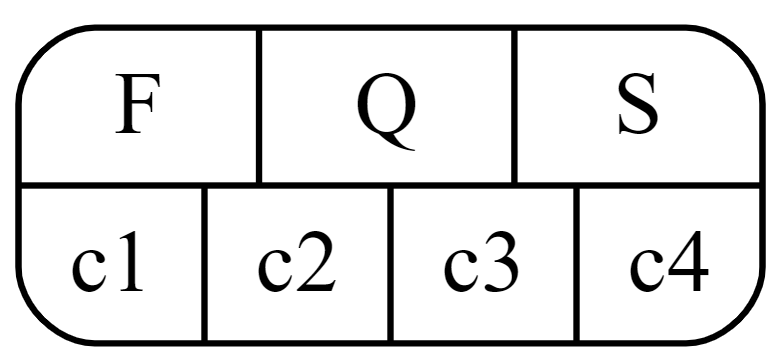
\includegraphics{C:/Users/zhuoh/Desktop/Docs/ds-21/数据结构与算法I 作业21.assets/image-20201223105222417.png}
\caption{}
\end{figure}

插入K:

\begin{figure}
\centering
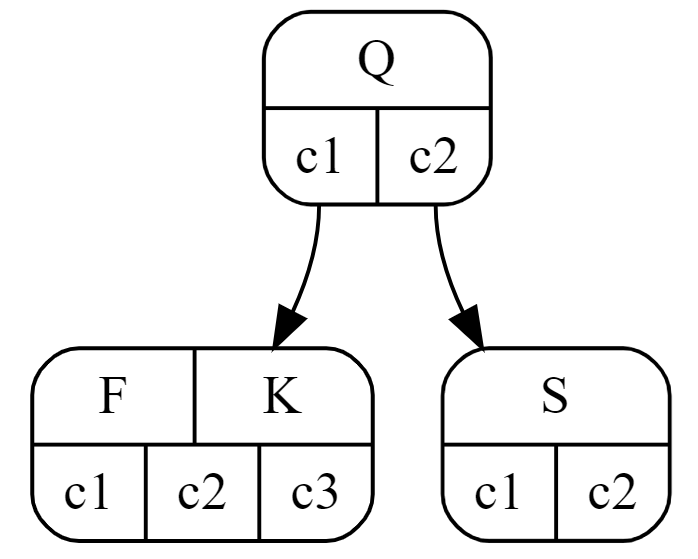
\includegraphics{C:/Users/zhuoh/Desktop/Docs/ds-21/数据结构与算法I 作业21.assets/image-20201223105502360.png}
\caption{}
\end{figure}

插入C:

\begin{figure}
\centering
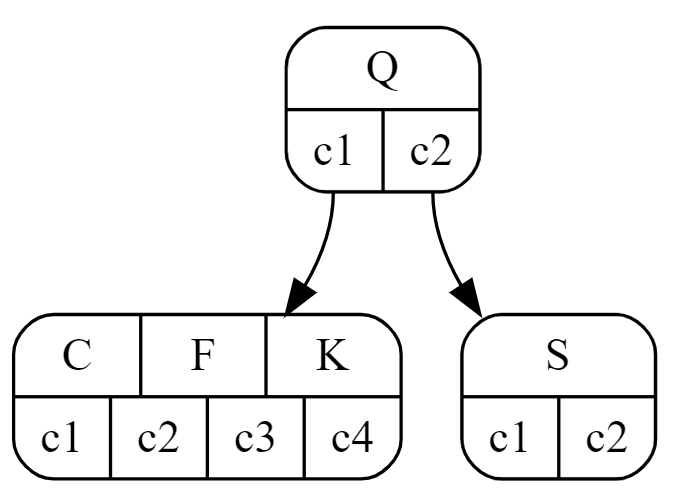
\includegraphics{C:/Users/zhuoh/Desktop/Docs/ds-21/数据结构与算法I 作业21.assets/image-20201223105544987.png}
\caption{}
\end{figure}

插入L:

\begin{figure}
\centering
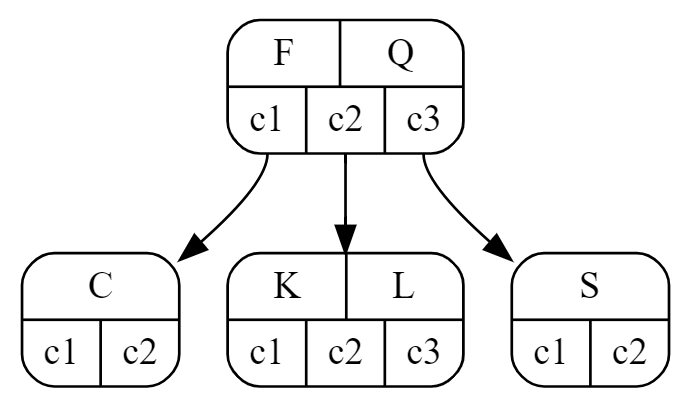
\includegraphics{C:/Users/zhuoh/Desktop/Docs/ds-21/数据结构与算法I 作业21.assets/image-20201223105836971.png}
\caption{}
\end{figure}

插入V后:

\begin{figure}
\centering
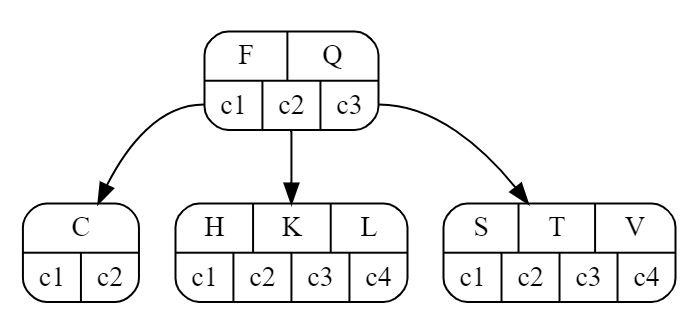
\includegraphics{C:/Users/zhuoh/Desktop/Docs/ds-21/数据结构与算法I 作业21.assets/image-20201223110130832.png}
\caption{}
\end{figure}

插入W后:

\begin{figure}
\centering
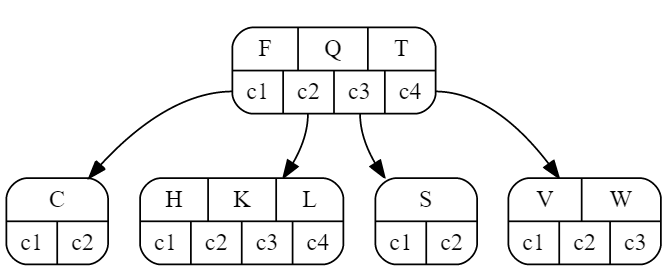
\includegraphics{C:/Users/zhuoh/Desktop/Docs/ds-21/数据结构与算法I 作业21.assets/image-20201223110307641.png}
\caption{}
\end{figure}

插入M前(分裂):

\begin{figure}
\centering
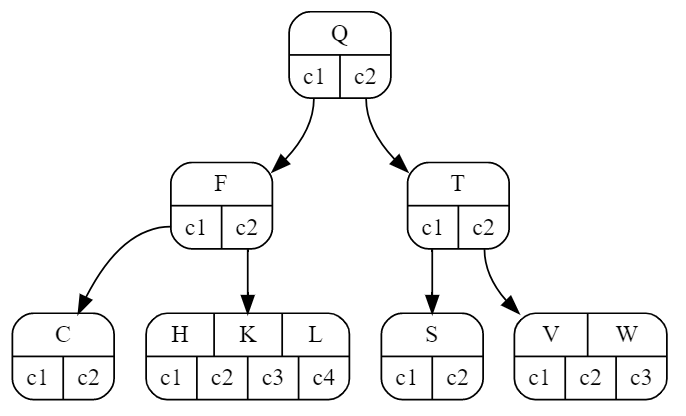
\includegraphics{C:/Users/zhuoh/Desktop/Docs/ds-21/数据结构与算法I 作业21.assets/image-20201223110946864.png}
\caption{}
\end{figure}

插入M后:

\begin{figure}
\centering
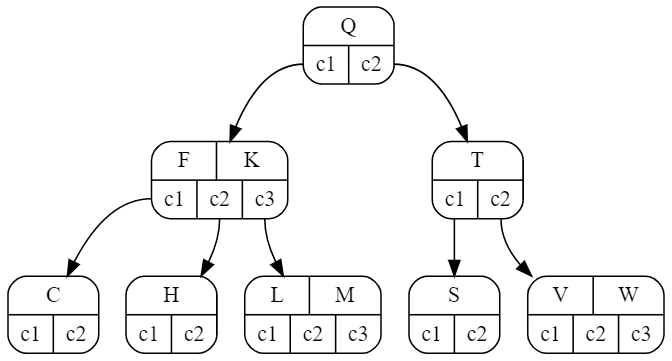
\includegraphics{C:/Users/zhuoh/Desktop/Docs/ds-21/数据结构与算法I 作业21.assets/image-20201223111138326.png}
\caption{}
\end{figure}

插入P后:

\begin{figure}
\centering
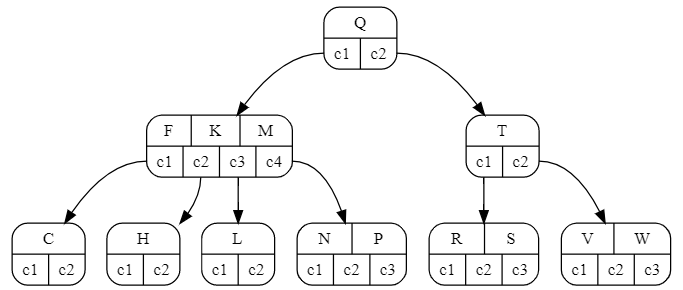
\includegraphics{C:/Users/zhuoh/Desktop/Docs/ds-21/数据结构与算法I 作业21.assets/image-20201223111514022.png}
\caption{}
\end{figure}

插入A前(分裂):

\begin{figure}
\centering
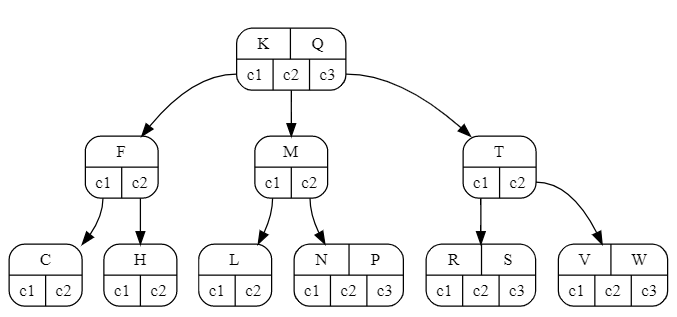
\includegraphics{C:/Users/zhuoh/Desktop/Docs/ds-21/数据结构与算法I 作业21.assets/image-20201223112013966.png}
\caption{}
\end{figure}

插入Y前(分裂):

\begin{figure}
\centering
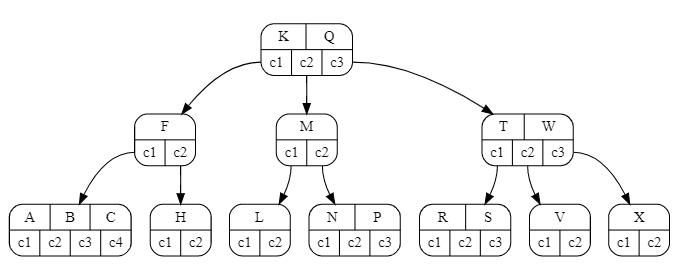
\includegraphics{C:/Users/zhuoh/Desktop/Docs/ds-21/数据结构与算法I 作业21.assets/image-20201223112319694.png}
\caption{}
\end{figure}

最终结果:

\begin{figure}
\centering
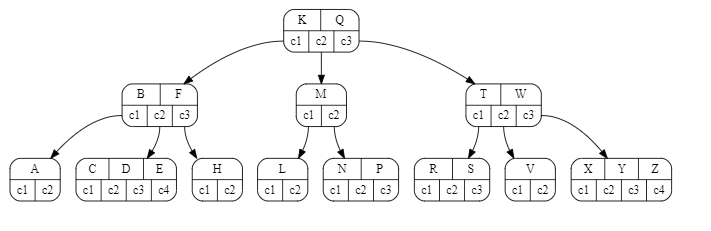
\includegraphics{C:/Users/zhuoh/Desktop/Docs/ds-21/数据结构与算法I 作业21.assets/image-20201223112618688.png}
\caption{}
\end{figure}

\hypertarget{header-n105}{%
\subsection{18.3-2}\label{header-n105}}

\begin{Shaded}
\begin{Highlighting}[]
\DataTypeTok{void}\NormalTok{ B_Tree_Delete(Node *x, }\DataTypeTok{int}\NormalTok{ k) \{}
\NormalTok{    B_Tree_Read(x);}
    \ControlFlowTok{if}\NormalTok{(x->leaf == }\KeywordTok{true}\NormalTok{) }
        \KeywordTok{delete}\NormalTok{ x->key[k];}
    \ControlFlowTok{else}\NormalTok{ \{}
        \ControlFlowTok{if}\NormalTok{(k in x->key[]) \{}
\NormalTok{            node *&y = find_predecessor(x, k), *&z = find_successor(x, k);}
\NormalTok{            node *kk = find_child(x, k);}
            \ControlFlowTok{if}\NormalTok{(y->size >= t) \{}
\NormalTok{                node *yy = find_predecessor(y, k);}
\NormalTok{                B_Tree_Delete(yy, k);}
\NormalTok{                y = yy;}
\NormalTok{            \}}
            \ControlFlowTok{else}\NormalTok{ \{}
                \ControlFlowTok{if}\NormalTok{(z->size >= t) \{}
\NormalTok{                    node *zz = find_successor(z, k);}
\NormalTok{                    B_Tree_Delete(zz, k);}
\NormalTok{                    z = zz;}
\NormalTok{                \}}
                \ControlFlowTok{else}\NormalTok{ \{}
                    \ControlFlowTok{if}\NormalTok{(z->size + y->size == }\DecValTok{2}\NormalTok{*t - }\DecValTok{1}\NormalTok{) \{}
\NormalTok{                        merge(y, kk, z);}
\NormalTok{                        x->key[].erase(kk), x->key.erase(z);}
\NormalTok{                        B_Tree_Delete(y, k);}
\NormalTok{                    \}}
\NormalTok{                \}}
\NormalTok{            \}}
\NormalTok{        \}}
        \ControlFlowTok{else}\NormalTok{ \{}
\NormalTok{            node *xk = Find_K_recursively(x, k), *xkf = xk;}
\NormalTok{            node *last = Find_father_of_xk(x, k);}
            \ControlFlowTok{if}\NormalTok{(xk->size == t - }\DecValTok{1}\NormalTok{ && (xk->left->size >= t || xk->right->size >= t)) \{}
\NormalTok{                xk->key.insert(last);}
                \ControlFlowTok{if}\NormalTok{(xk->left->size >= t) x->key.insert(xk->left);}
                \ControlFlowTok{else}\NormalTok{ x->key.insert(xk->right);}
\NormalTok{            \}}
            \ControlFlowTok{if}\NormalTok{(xk->size == t - }\DecValTok{1}\NormalTok{ && xk->left->size == t - }\DecValTok{1}\NormalTok{ && xk->right->size == t - }\DecValTok{1}\NormalTok{) \{}
\NormalTok{                merge(xk->left, last, xk);}
\NormalTok{            \}}
\NormalTok{            B_Tree_Delete(last, k);}
\NormalTok{        \}}
        
\NormalTok{    \}}
\NormalTok{    B_Tree_Write(x);}
\NormalTok{\}}
\end{Highlighting}
\end{Shaded}

\end{document}
